\appendix
This document provides a list of supplemental materials that accompany the main paper.
\begin{itemize}
    \item \textbf{Part Segmentation Visualization} - We sample shapes from test set and visualize our predictions (see $part\_segmentation\_visualization.mov$ file). Notice the experiment is conducted on complete shapes, as is described in ``Per-category shape part segmentation'' in Section $5.2$ of the main paper.
    \item \textbf{SpecTN Initialization} - We discuss technical details about how we initialize SpecTN including how we generate a set of pre-computed functional maps (see Section~\ref{sec:init}).
    \item \textbf{Implementation Details} - We describe implementation details as well as hyperparameter choices in Section~\ref{sec:impl}.
    \item \textbf{Partial Shape Part Segmentation} - We provide additional per-category IoU for partial shape part segmentation task and compare our approach with ACNN~\cite{boscaini2016learning} in Section~\ref{sec:partial}.
    \item \textbf{Robustness to Sampling Density Variation} - We show the robustness of our approach w.r.t point cloud density variation in Section~\ref{sec:robustness}.
    \item \textbf{Normal Prediction} Another graph vertex function prediction task is conducted in Section~\ref{sec:normal} to validate the generalizability of our approach to very local properties. We predict shape vertex normals and the results are visualized in Figure~\ref{fig:normpred}.
\end{itemize}

\section{SpecTN Initialization}
\label{sec:init}
A set of precomputed functional maps are used for SpecTN pre-training. We mentioned in the main paper that the functional map $C$ from $\shape$ to the average shape $\bar{\shape}$ could be induced from the spatial correspondences between $\shape$ and $\bar{\shape}$, by the primal-dual relationship. Once we have the bases of $\shape$ and $\bar{\shape}$, as well as the rough spatial correspondences between them from the volumetric occupancy, the functional map can then be discovered by the approach proposed in \cite{ovsjanikov2012functional}. 

To be specific, we use $\myvec{B}_v$ to denote the volumetric reparametrization of graph laplacian eigenbases $\myvec{B}$ for each shape $\shape$, and use $\bar{\myvec{B}}_v$ to denote the grahp laplacian eigenbases of $\bar{\shape}$. $\myvec{B}_v$ and $\bar{\myvec{B}}_v$ both lie in the volumetric space and their spatial correspondence is natural to acquire. The functional map $C_{pre}$ aligning $\myvec{B_v}$ with $\bar{\myvec{B}}_v$ could be computed through simple matrix multiplication $C_{pre}=\bar{\myvec{B}}_v^T\myvec{B}_v$. The computed functional map will serve as supervision and SpecTN is pretrained to minimize the loss function $||C-C_{pre}||_F^2$.

It is worth mentioning that, if the shapes under consideration are diverse in topology and geometry, i.e. shapes from different categories, aligning every shape to a single ``average'' shape might cause unwanted distortion. Therefore we leverage multiple ``average'' shapes $\{\bar{\shape}_i\}_{i=1}^{n}$ and use a combination of their spectral domains as the canonical domain. Specifically, we assign each shape $\shape$ to its closest ``average'' shape under some global similarity measurement (i.e. lightfield descriptor) and use $\{a_i\}_{i=1}^n$ to represent such assignment, namely $a_i=1$ if $\shape$ is assigned to $\bar{\shape}_i$ and $a_i=0$ otherwise. Also we use $\bar{\myvec{B}}_{vi}$ to denote the spectral bases of $\bar{\shape}_i$. Then the functional map $C_{pre}$ for each shape $\shape$ could be computed through $C_{pre}=[a_1\bar{\myvec{B}}_{v1} \;a_2\bar{\myvec{B}}_{v2}\; ...\; a_n\bar{\myvec{B}}_{vn}]^T\myvec{B}_v$. The SpecTN is pretrained to predict a functional map which only synchronizes spectral domain of each shape to its most similar ``average'' shape.

\section{Implementation Details}
\label{sec:impl}
In most of our experiments, input shapes are represented as point cloud with around $2000-3000$ points. Given an input shape point cloud, we build a k-nearest neighbor graph $\graph$ first. We use $k=6$ in all our experiments. Then a graph weight matrix $W$ could be constructed in which $W_{i,j}=\frac{1}{d_{i,j}^2}$ if point $i$ and $j$ are connected, $0$ otherwise. We then compute the symmetric normalized graph laplacian $L$ as $L=I-D^{-1/2}WD^{-1/2}$, where $D$ is the degree matrix and $I$ denotes identity matrix. Since many natural functions we care about could be depicted by a small number of low-frequency laplacian eigenbases, we compute and use the smallest $100$ eigenvalues as well as the corresponding eigenbases for each $L$ in all our experiments. 

The choice of dilation parameters $\gamma$, number of output channels after each convolution layer, number of learnable parameters in each convolution kernel are shown in Table~\ref{tab:architecture}. We choose $c=50$ in all of our experiments. As is mentioned, we only consider the problem of synchronizing the low-frequency end of different spectral domains, so we choose to predict a functional map $C\in\mathbb{R}^{15\times45}$ in all our experiments, which maps the first $15$ eigenbases of each individual spectral domain into a canonical domain of dimension $45$. Notice the dimension of canonical domain is larger that each individual domain to allow very different shapes to be mapped into different subspaces.

\begin{table}[]
\centering
{\footnotesize
\begin{tabular}{@{}p{0.25\linewidth}p{0.015\linewidth}p{0.015\linewidth}p{0.015\linewidth}p{0.015\linewidth}p{0.015\linewidth}p{0.015\linewidth}p{0.017\linewidth}p{0.016\linewidth}p{0.016\linewidth}p{0.015\linewidth}}
\toprule
Layer               & 1  & 2  & 3  & 4  & 5  & 6  & 7   & 8   & 9  & 10 \\ \midrule
Dilation ($\gamma$) & 1  & 1  & 4  & 4  & 16 & 16 & 64   & 64   & 1  & 1  \\
SpecTN              & No & No & No & No & No & No & Yes & Yes & No & No \\
\#Kernel Param      & 7  & 1  & 7  & 1  & 7  & 1  & 45  & 45  & 7  & 1  \\
\#Out Channel    & c  & c  & c  & c  & 2c & 2c & 2c  & 2c  & 2c & 2c\\ \bottomrule
\end{tabular}
}
\caption{Parameters used in different layers of the architecture, including dilation parameter $\gamma$ which controls convolution kernel size, whether use spectral transformer network (SpecTN), the number of learnable parameters in convolution kernels, the number of output channels after each convolution operation.}
\label{tab:architecture}
\end{table}

\section{Partial Shape Part Segmentation}
\label{sec:partial}
We provide per-category IoU for partial shape part segmentation experiments in this section, which is not included in the main paper due to space limit. We compare our approach with baseline method ACNN \cite{boscaini2016learning} and the results are shown in Table~\ref{tab:partialsegmore}

Notice our approach outperforms ACNN on most categories and the margin between ACNN and ours is large on average. Our approach is also more robust to data incompleteness since its performance drop from complete data segmentation results is less significant than ACNN.

\begin{table*}[t!]
\centering
\small
\begin{tabular}{@{}p{0.04\linewidth}|p{0.05\linewidth}p{0.07\linewidth}|p{0.025\linewidth}p{0.022\linewidth}p{0.022\linewidth}p{0.022\linewidth}p{0.025\linewidth}p{0.025\linewidth}p{0.025\linewidth}p{0.025\linewidth}p{0.025\linewidth}p{0.025\linewidth}p{0.025\linewidth}p{0.025\linewidth}p{0.025\linewidth}p{0.025\linewidth}p{0.025\linewidth}p{0.025\linewidth}}
\hline
& mean partial & mean complete & plane & bag & cap & car & chair & ear-phone & guitar & knife & lamp & laptop & motor-bike & mug & pistol & rocket & skate-board & table \\ \hline
ACNN & 69.21 & 79.63 & 62.73 & 63.26 & 58.90 & 38.25 & 70.59 & \textbf{68.68} & \textbf{88.08} & 74.58 & 61.49 & 87.03 & 31.90 & 79.92 & 62.98 & 35.70 & 68.41 & 76.07 \\ \hline
Ours1 & 76.19 & 83.48 & 71.01 & 77.61 & 64.78 & 56.05 & 78.97 & 68.50 & 84.63 & 82.01 & 73.02 & 91.40 & 40.71 & 87.34 & 72.60 & \textbf{42.53} & 80.61 & 79.55 \\
Ours2 & \textbf{78.02} & \textbf{84.74} & \textbf{74.55} & \textbf{82.58} & \textbf{65.36} & \textbf{58.12} & \textbf{80.41} & 65.55 & 84.75 & \textbf{82.53} & \textbf{77.39} & \textbf{93.15} & \textbf{43.12} & \textbf{90.24} & \textbf{74.71} & 42.17 & \textbf{83.22} & \textbf{80.51} \\ \hline
\end{tabular}
\caption{IoU for part segmentation on incomplete shapes. Note that for comparison, we not only report mean IoU for partial shape part segmentation under ``mean partial'', but also list mean IoU for complete shape part segmentation under ``mean complete''. Ours1 represents a variation of our framework without SpecTN and Ours2 corresponds to our full pipeline with SpecTN. On average we outperform ACNN, the baseline approach, by a large margin and we outperforms ACNN on most shape categories. Moreover, our approach is more robust to data incompleteness since its performance drop is lower in comparison with complete shape segmentation.}
\label{tab:partialsegmore}
\end{table*}

\section{Robustness to Sampling Density Variance}
\label{sec:robustness}
In this experiment, we evaluate the robustness of our approach w.r.t point cloud density variation. To be specific, we train our SyncSpecCNN for shape segmentation on the point cloud provided by \cite{Yi16} first. Then we downsample the point cloud under different downsample ratio and evaluate our trained model to check how segmentation performance would change. Again we evaluate our approach with/without SpecTN and the result is shown in Figure~\ref{fig:downsample}.
 
By introducing SpecTN, our framework becomes more robust to sampling density variation. Our conjecture is that sampling density variation may result in large spectral space perturbation, therefore being able to synchronize different spectral domains becomes especially important.

\begin{figure}
 \centering
 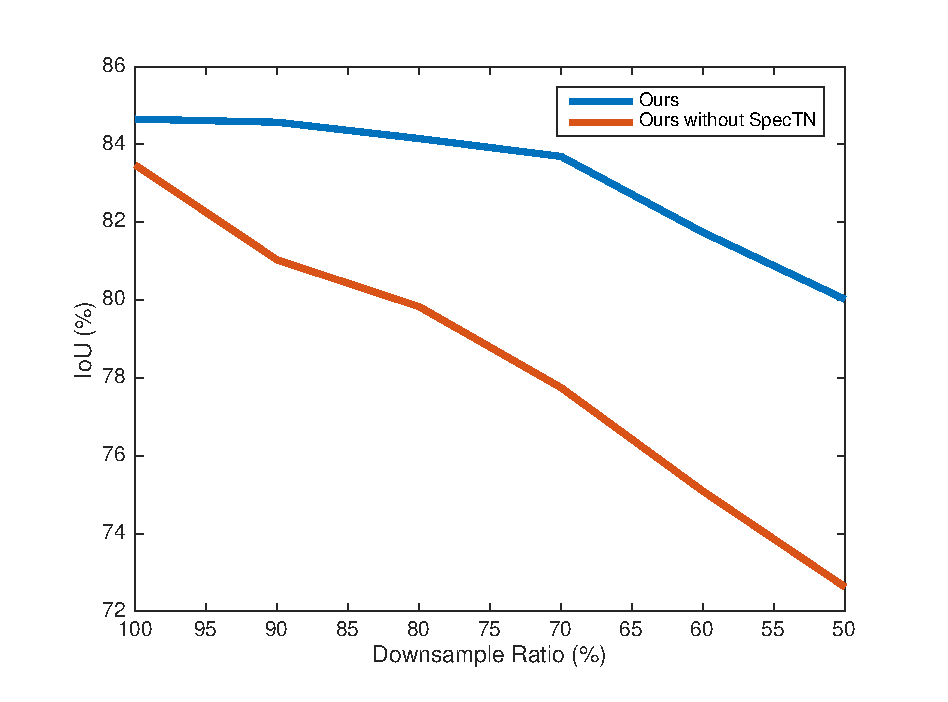
\includegraphics[width=0.75\linewidth]{./fig/downsample.eps}
 \caption{We evaluate the robustness of our model to sampling density change. Test shapes are downsampled by different ratios and fed into our network. We compute the segmentation IoU for different downsample ratios and show it here. With SpecTN, our framework becomes more robust to sampling density change.}
 \label{fig:downsample}
\end{figure}

\section{Normal Prediction}
\label{sec:normal}
Our framework could learn generic graph functions not limited to part segmentation or keypoint prediction. To validate this point, we leverage our proposed SyncSpecNet to learn another type of graph vertex function, vertex normal function. Specifically, our SyncSpecNet takes the XYZ coordinate function of graph vertices as network input and predicts vertex normal as output. The network is trained to minimize the L2 loss between ground truth normals and predicted normals. We use the official train/test split provided by \cite{shapenet2015} and visualize some of the normal prediction results from test set in Figure~\ref{fig:normpred}.

\begin{figure}
 \centering
 \includegraphics[width=1\linewidth]{./fig/visnormal.pdf}
 \caption{We evaluate our framework on normal prediction task. The colors shown on the 3D shape are RGB-coded normals, namely putting XYZ components of normal directions into RGB channels. Our framework could predict reasonable normal directions even on very thin structures.}
 \label{fig:normpred}
\end{figure}

It can be seen our predictions are very close to the ground truth at most of the time.Even on thin structures the normal predictions are still reasonable. One problem of our prediction is that it tends to generate smoothly transiting normals along the boundary while the ground truth is sharper. This is due to the fact that we are using a small number of eigenbases in our experiments, which is not friendly to regression tasks with very high frequency signal as target.